
\chapter{Summary and outlook}
\label{chap:summary}

%COFI -- chapter outline and flow integration\\

% already in chapters:\\
% results\\
% discussion\\
% conclusions\\
% 
% end matter:\\
% summary\\
% outlook\\

\section{Summary}

% long synopsis chapter2 without refs
long synopsis chapter2 without refs\\

% long synopsis chapterPSP without refs
long synopsis chapterPSP without refs\\

% results summary handout
results summary handout\\
- equations and under which circumstances they are to be used\\



In order to derive the link from near-Earth solar wind properties to its \Kp{}~impact, 35~years of solar wind high-resolution measurements were correlated with the \Kp~index and empirical relations were derived that enable the prediction of \Kp{} from the solar wind velocity and the IMF z"~component. Early predictions of CME and ambient stream magnetic fields obtained from near-Sun observations currently either are not existent or come with high uncertainties. Thus, to provide \Kp{} predictions, I derived relations exclusively from their arrival velocity.\\


I built an empirical solar wind model for the inner heliosphere in the ecliptic which accounts for the variations of the solar activity cycle and for solar distance. In order to obtain empirical estimates of the solar wind environment PSP is to encounter, this solar wind model is extrapolated down to PSP's planned near-Sun perihelia and is built to consider the expected solar activity during PSP's mission.\\



\section{Outlook}

feed from outlooks...\\

The present study adds more empirical \Kp{} relations -- for the cases when only the solar wind velocity $v$ or its electric field \vBz{} are known, see \autoref{chap:chapter2}. The derived \Kp{} relations are the last part of the UGOE/IAG CME forecast chain.\\

Using the SSN prediction, the derived solar wind model allows the forecast and extrapolation of the solar wind environment occuring during the PSP mission's near-Sun encounters from end of 2018 on. The anticipated Parker~Solar~Probe data (near-Sun measurements) will reveal how far the solar wind estimates really are from reality and thus is able to locate the outer boundary of the solar wind acceleration region.\\

DSCOVR data (advantages over ACE? gain?)\\

other possible spacecraft missions that would be beneficial for space weather forecasting: sub-L1 for earlier in-situ CME magnitude warning (cite?) and L5 for early CME velocity and arrival warning \citep{Vourlidas2015}\\


%german version of summary






\section{notes...}

put fig. somewhere earlier (p.~10?): see \autoref{fig:Hundhausen1977_fig20bcd}\\
\begin{figure}[htb]
	\centering
	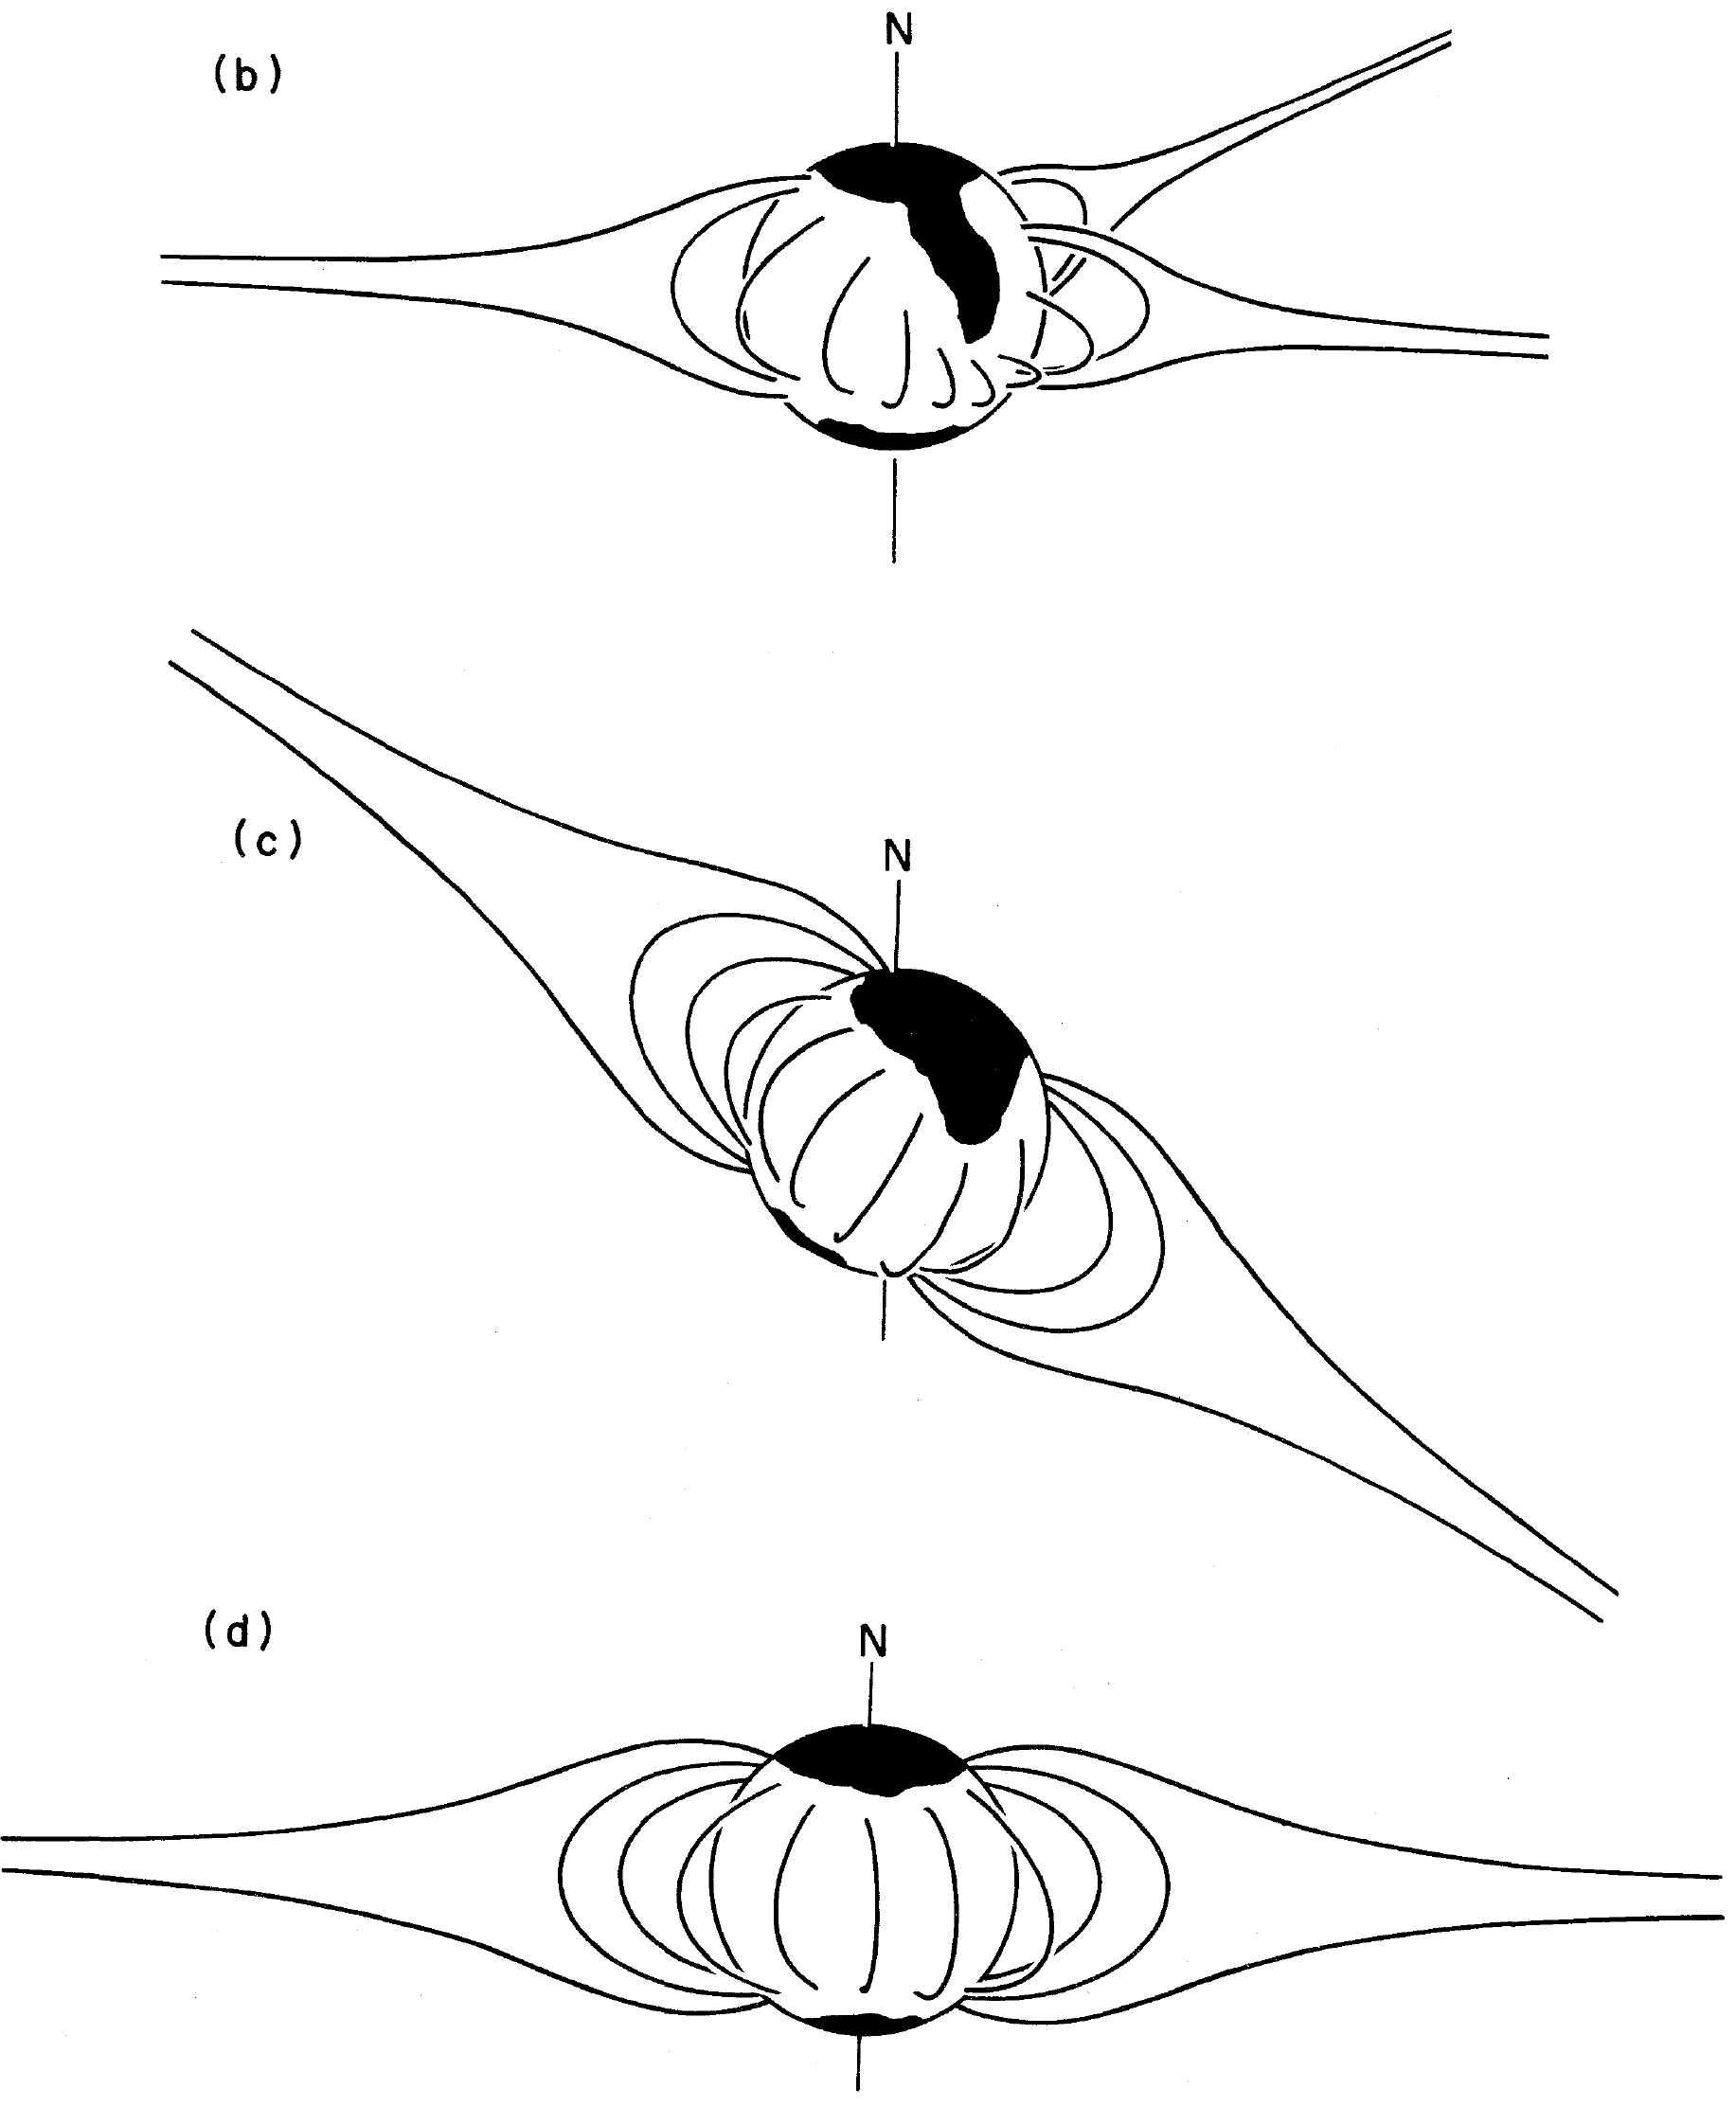
\includegraphics[width=0.5\textwidth]{figures_of_others/images/Hundhausen1977_fig20bcd.png}
	\caption[\lofimage{figures_of_others/images/Hundhausen1977_fig20bcd.png}Credit: {\citep[Fig.~20, panels (b--d)]{Hundhausen1977}}, \textcopyright~Colorado Associated University Press, reproduced with permission.]
	{Schemata of different coronal configurations during the solar cycle. Visualized are the locations of closed coronal magnetic fields (lines) and coronal holes (black areas) for a post maximum distorted dipole (top panel), for a pre minimum stable tilted dipole (middle panel), and a post minimum axial dipole (bottom panel). Credit: {\citep[Fig.~20, panels (b--d)]{Hundhausen1977}}, \textcopyright~Colorado Associated University Press, reproduced with permission.}
	\label{fig:Hundhausen1977_fig20bcd}
\end{figure}

causes (see citet{Rangarajan1997} p.~1282 and mention Bartels1963 too)\\

\citet{Sonnerup1967}: The rotational discontinuity seems to occur predominantly during magnetic storms and two of these cases, involving substantial normal-field components, provide compelling evidence that field reconnection takes place during the storm main phase.\\

% mass flux considerations:\\
% mass per second per Earth disc...\\
% R_E = 6371.008 km\\
% A_E = pi * R_E² = 127 516 438.219 km²\\
% m_p = 1.672621898e-27 kg\\
% v = 400 km/s\\
% n = 6.5 cm-3 = 6.5e15 km-3\\
% mass flux_E = m_p * n * v * A_E = 0,554538384917 kg/s\\
% = 555 g/s = 1996 kg/h = 48 t/d = 17487 t/a\\
% mass per second per magnetosphere disc...\\
% R_MP = 15 * R_E
% A_MP = pi * R_MP² = 28 691 198 599.3 km²\\
% mass flux_MP = 124,772770348 kg/s\\
% = 449 t/h = 10 780 t/d = 3 934 834 t/a\\

% Wikipedia: https://en.wikipedia.org/wiki/Solar_wind
% The wind exerts a pressure at 1 AU typically in the range of 1–6 nPa (1–6×10−9 N/m2), although it can readily vary outside that range.
% The ram pressure is a function of wind speed and density. The formula is
% P = mp * n * V2= 1.6726×10−6 * n * V2
% where mp is the proton mass, pressure P is in nPa (nanopascals), n is the density in particles/cm3 and V is the speed in km/s of the solar wind.[citation needed]

% HCS
why HCS? what currents are there...\\
why is the CS not the divide between both polarities?\\

% space weather
"The principal users affected by geomagnetic storms are the electric power grid, spacecraft operations, users of radio signals that reflect off of or pass through the ionosphere, and observers of the aurora." NOAA cite\\

strong radio bursts; are they relevant direct disturbances for space weather?\\

The solar wind total energy flux at Earth ($1.45~\text{mW/m}^2$) is only about one millionth of the solar radiation flux at Earth (see \citet[p.~153]{Schwenn1990}).\\

% magnetosphere
Phan2005, Magnetopause Processes:\\
Cluster findings include:\\
A strong ‘guide field’ detected at a reconnection X-line, i.e., a finite magnetic field along the X-line, has provided direct evidence for component merging.\\
Tailward-of-the-cusp reconnection has been found to occur only when the IMF has a northward component. The occurrence rate of cusp reconnection is nearly 100\% when the IMF has a northward component, implying that cusp reconnection in the northern and southern hemispheres must be common. The high occurrence rate (in contrast to a rate of 50\% at the subsolar magnetopause) is thought to be due to the presence of a plasma depletion layer. In this layer, the plasma beta is reduced, rendering the magnetosheath flow sub-Alfvenic and allowing the establishment of a stable X-line at the high-latitude magnetopause.\\

look into printed paper collection...\\

% geomagnetic indices
\citet{Lockwood2014} even used geomagnetic indices (including $aa$) to reconstruct the near-Earth IMF strength and solar wind flow speed back to 1845.\\

% halo CMEs:
observed coronal transient: 3d structure, directed at Earth, associated with shock wave; \citep{Howard1982} -> halo CME\\

% chapter2
This work adopts these assumptions and treats the solar wind throughout as a proton plasma.\\

% Kp forecast models
% Aleksei's f/c model; Ukraine; developed within AFFECTS project Space Research Institute of NAS of Ukraine and SSA of Ukraine, Ukraine (SRI NASU-NSAU)\\
% http://www.ikd.kiev.ua/index.php?option=com_content&view=article&id=22%3A2011-02-09-12-19-54&catid=12&Itemid=15&lang=en

% The $\text{d}\Phi / \text{d}t$ coupling relation is being implemented into CME forecast procedures \citep{Savani2017}.\\
% NASA's Space Weather Research Center (SWRC); the derived Kp estimates using real-time in-situ data from L1 are currently implemented within the CCMC integrated Space Weather Analysis System (iSWA); Community Coordinated Modeling Center (CCMC) at the Goddard Space Flight Center\\

% coupling functions
\citet{Elliott2013}: The \Kp~index and solar wind speed relationship: Insights for improving space weather forecasts\\

% Kp index
There exist several indicators/quantities that scale or are based on the \Kp{}~index:
\begin{itemize*}
	\item The equatorward auroral boundary position correlates with the \Kp~index (cite?).
	\item The variation of the total electron content (TEC) of the ionosphere correlates with the \Kp~index (cite?). The TEC has influence on global navigation satellite systems (GNSS). A part of their positional error scales directly with TEC (in extreme cases up to about \SI{30}{\m}).
\end{itemize*}

% solar wind impacts
These solar wind real-time data are used to nowcast various effects on the Earth's magnetosphere, such as the position of the magnetospheric bow shock in front of the Earth, the magnitude of geomagnetic disturbances, the positions of the polar auroral ovals, the variation of the total electron content (TEC) of the ionosphere, and the positional error of global navigation satellite systems (GNSS).\\


